\chapter{步兵项目}
\label{ch:concise-infantry}

\begin{introduction}
  \item 配置遥控器通道、死区与四轮底盘；
  \item 配置云台两个轴、拨弹电机与摩擦轮；
  \item 分配按键并完成方向校准；
  \item 完成检查、编译、烧录与首次上车核对。
\end{introduction}

步兵项目是校内赛最常用的构型：四轮底盘负责移动，云台负责瞄准，拨弹电机把弹丸送入
摩擦轮，摩擦轮把弹丸射出。向导共六步：遥控器与底盘、云台与拨弹、控制与摩擦轮、
检查与摘要、生成代码、烧录。

\section{遥控器与底盘}

\subsection{手柄与通道号}

智能交互手柄通过无线模块与主控板通信，面板包括左右摇杆、A--E 字母按键、四个方向键、
重置键与通道号查看键（图~\ref{fig:concise-handle}）。两只摇杆本身也可以按下，分别记作
LC 与 RC；摇杆的水平与竖直方向提供 LX、LY、RX、RY 四个轴输入。

\begin{figure}[htbp]
  \centering
  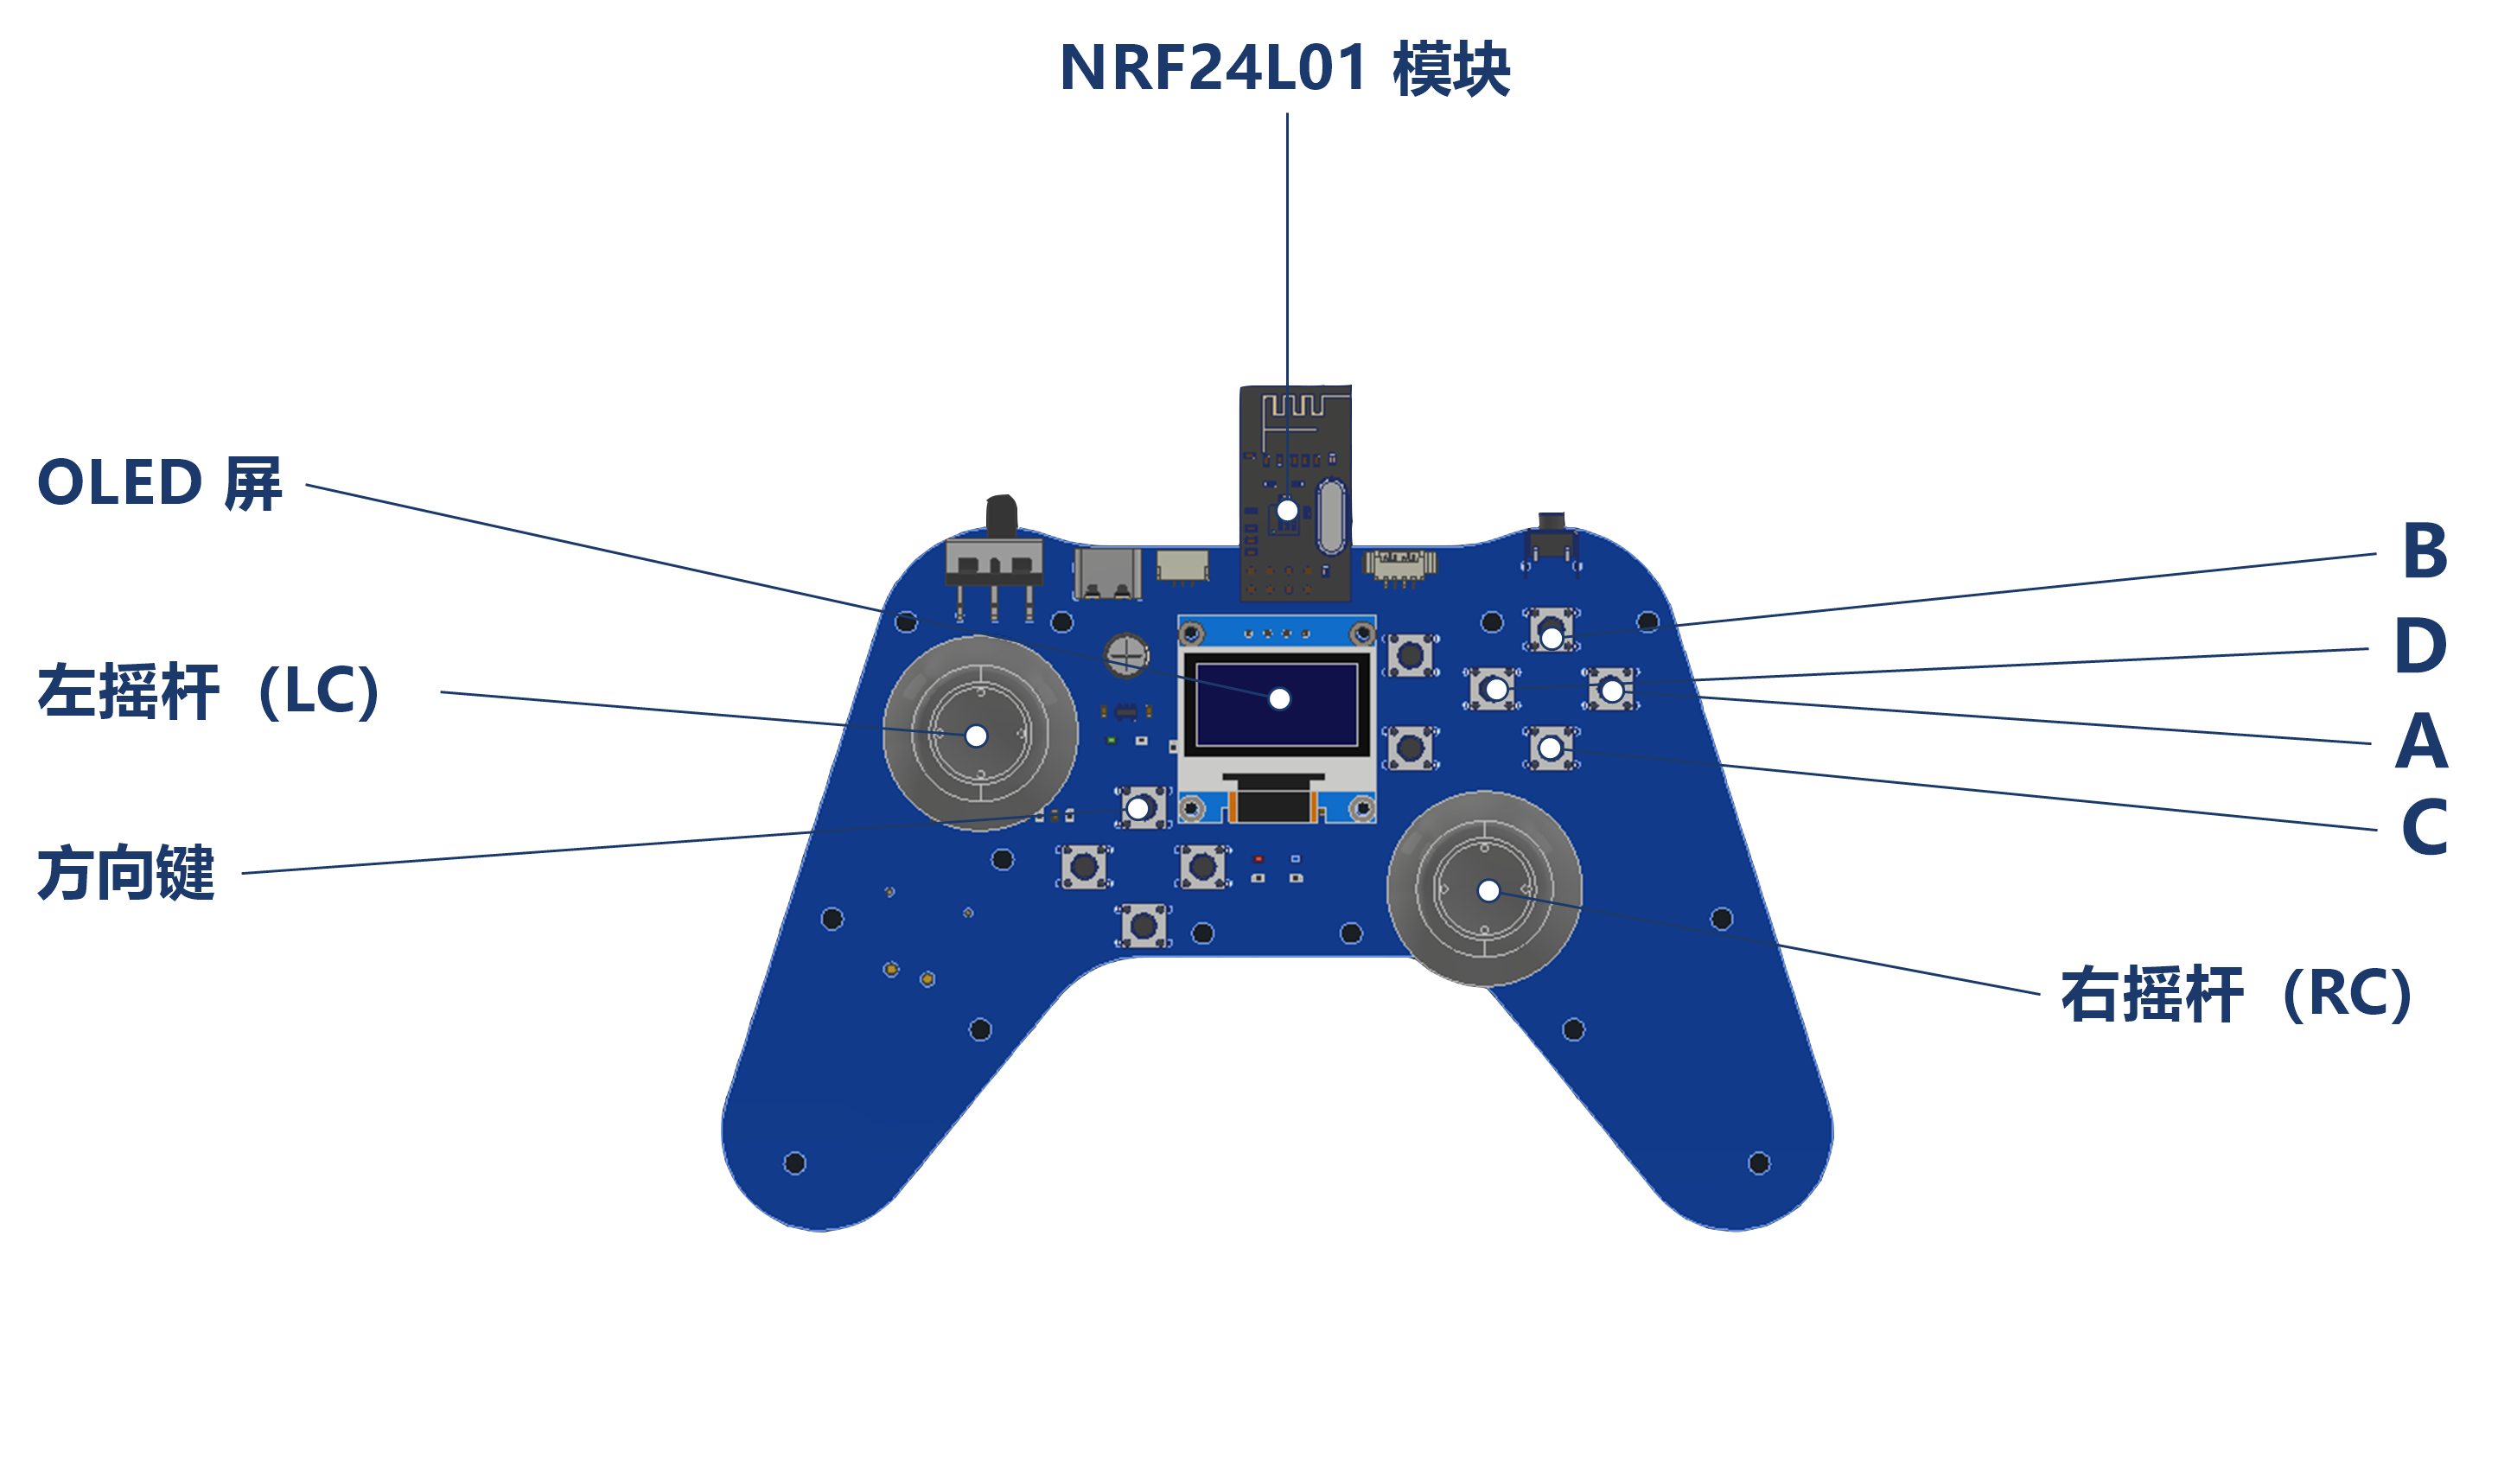
\includegraphics[width=0.98\linewidth]{image/ch03/handle-layout.png}
  \caption{智能交互手柄面板：双摇杆、字母按键、方向键与 OLED 屏}
  \label{fig:concise-handle}
\end{figure}

手柄与主控板必须使用同一个通道号。手柄开机后长按通道号查看键，屏幕显示当前通道号；
把该数字填入“遥控器与底盘”页的“通道号”一栏即可。通道不一致时主控板收不到任何数据，
这是“车完全不动”的首要排查项。

“摇杆死区”用于忽略摇杆回中后的微小偏移。死区太小，底盘可能在无操作时缓慢漂移；死区
太大，小幅推杆没有反应，操控显得迟滞。取值范围为 0--2047，建议不超过 500，100 是常用
的起始值。

\subsection{四轮与方向}

“四轮底盘”区按左前、左后、右前、右后分别选择 IO 与方向
（图~\ref{fig:concise-remote}）。IO 下拉框只列出当前可用的电机端口；同侧前后轮可以共用
一个 IO，但共用时两轮方向必须相同。

\begin{figure}[htbp]
  \centering
  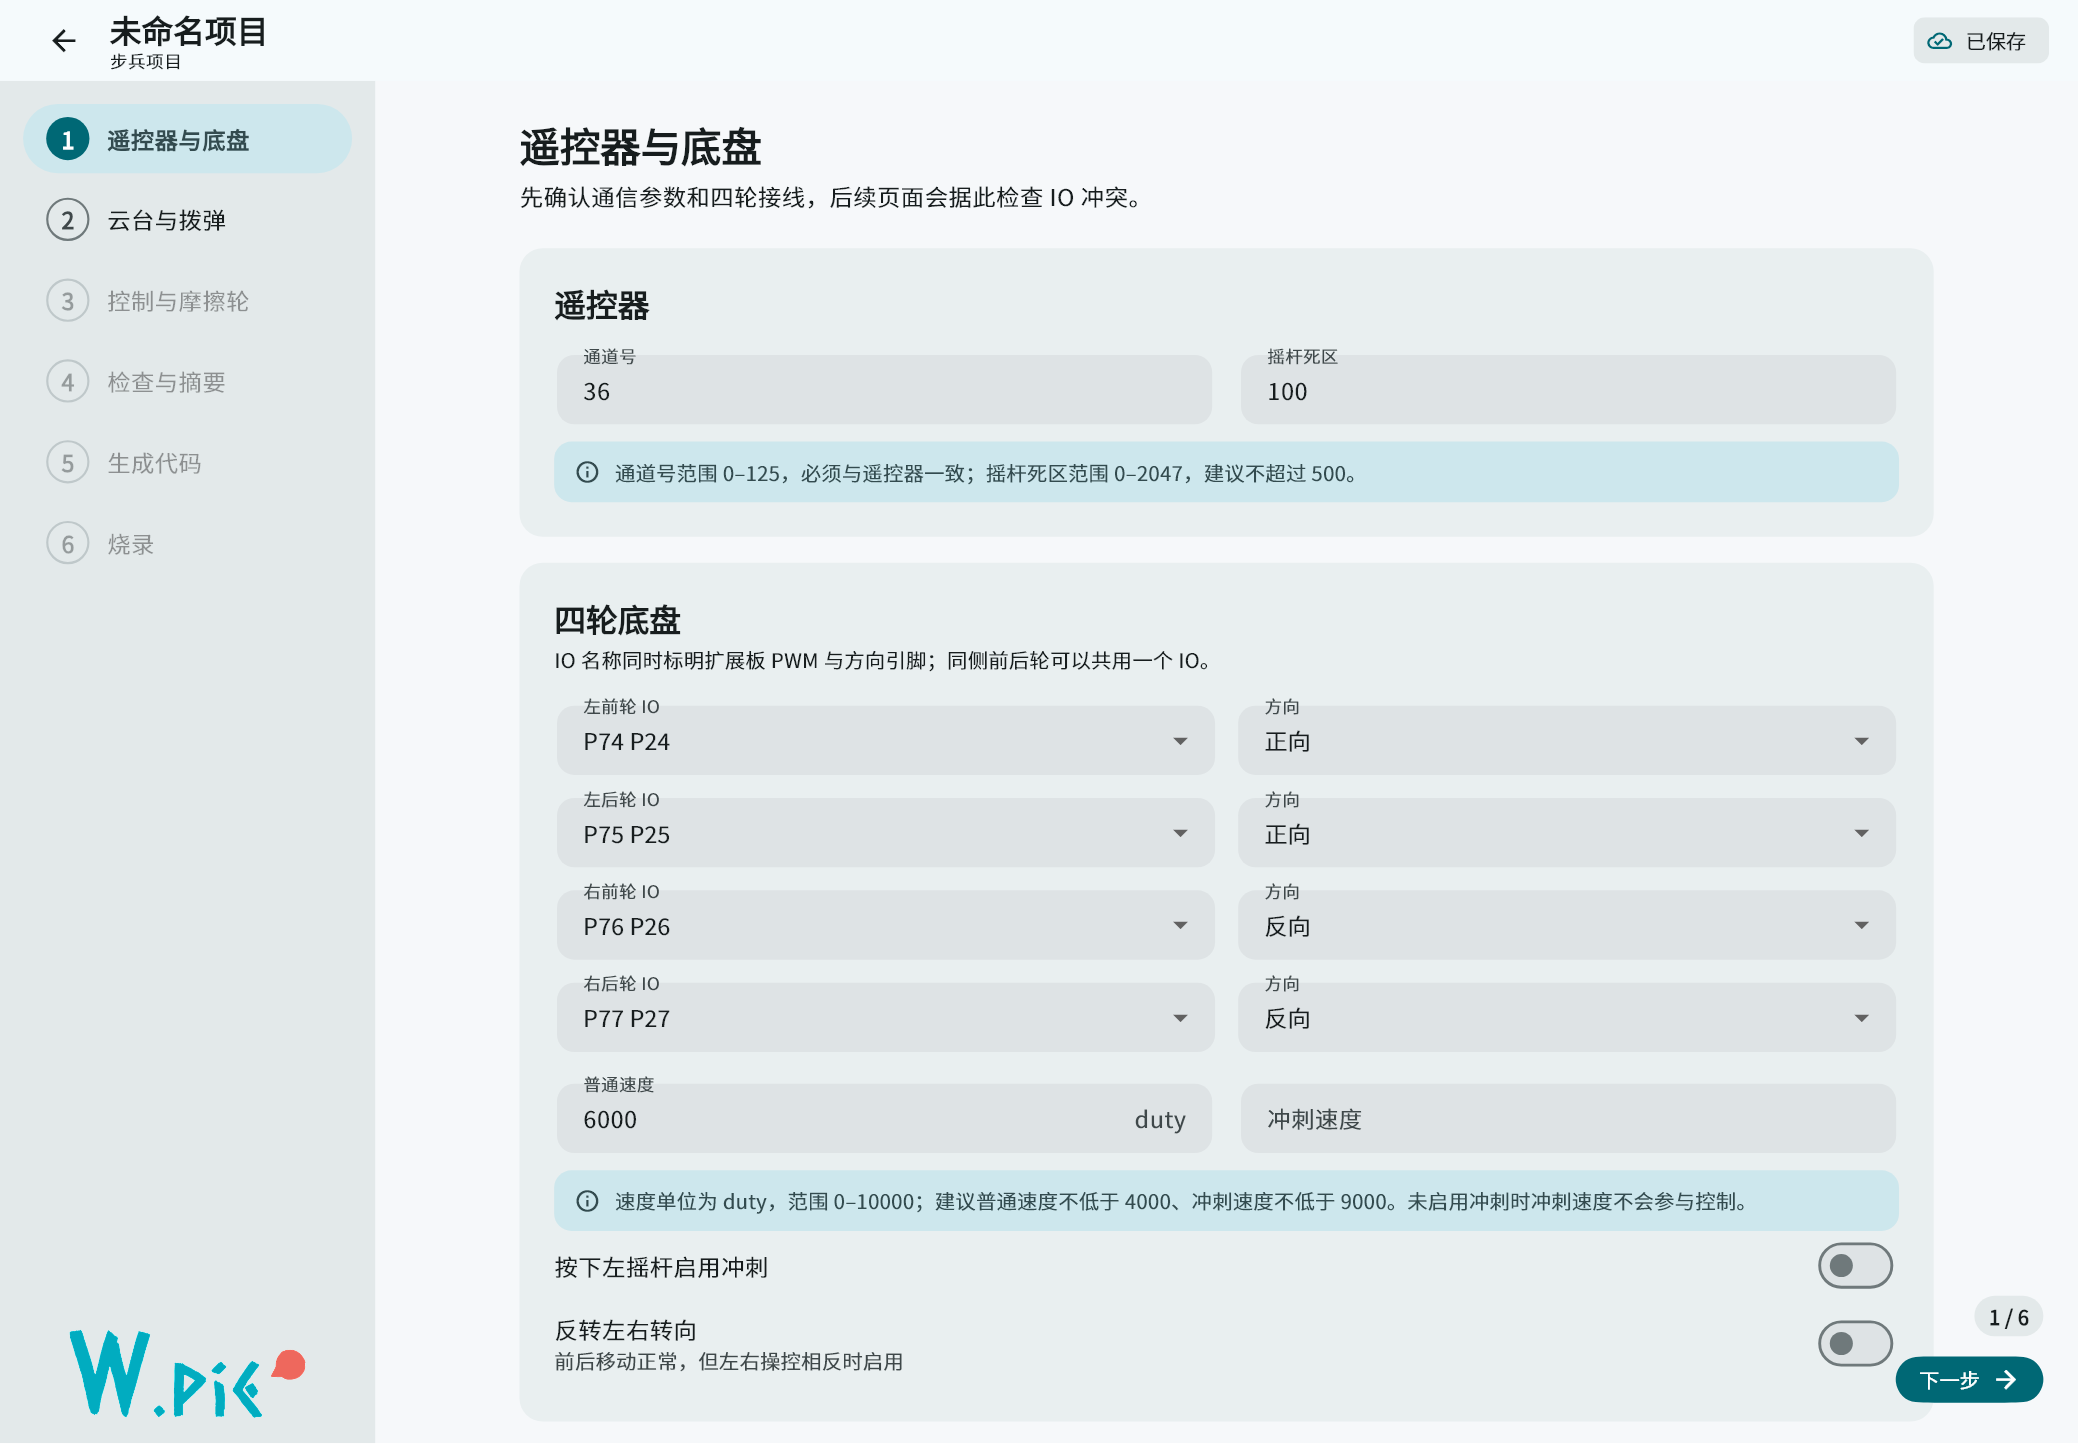
\includegraphics[width=0.98\linewidth]
    {image/ch03/3-1-remote-top.png}
  \caption{“遥控器与底盘”页：通道、死区、四轮 IO 与方向、普通与冲刺速度}
  \label{fig:concise-remote}
\end{figure}

“方向”表示该路电机的安装与接线是否符合默认约定。最常见的情形是右侧电机镜像安装，
因此右侧两轮通常设为“反向”，左侧两轮设为“正向”。装配后若某个轮子的转向与预期相反，
修改该轮的方向即可，不需要更改接线。

\subsection{速度与操控}

“普通速度”是左摇杆推满时的底盘速度，建议不低于 4000；“冲刺速度”是按住冲刺键时的
速度，建议不低于 9000，且不得小于普通速度。两者取值范围均为 0--10000。

打开“按下左摇杆启用冲刺”后，按下左摇杆即切换到冲刺速度，松开恢复普通速度。若前后
移动正常、左右转向相反，打开“反转左右转向”即可，不必改动电机接线。

\subsection{方向校准}

首次上车按下述顺序核对，全程架空并临时降低普通速度：

\begin{enumerate}
  \item 轻推左摇杆向上，四个轮子应同时向前滚动；某个轮子相反时，修改该轮的方向；
  \item 轻推左摇杆向左，车体应向左转；方向相反时，打开“反转左右转向”；
  \item 按下左摇杆并推满，速度应明显提升；
  \item 确认无误后落地，低速试走直线，再逐步提高速度。
\end{enumerate}

\section{云台与拨弹}

\subsection{云台两个轴}

“云台与拨弹”页把云台分为 Yaw（偏航，水平旋转）与 Pitch（俯仰）两个轴
（图~\ref{fig:concise-mechanism}）。每个轴默认有一个执行器，点击“添加执行器”可以扩展为
多个执行器同步动作。每个执行器填写四项：

\begin{itemize}
  \item \textbf{驱动类型}：舵机或电机；IO 下拉框只给出该类型可用的端口；
  \item \textbf{IO}：执行器所在端口；
  \item \textbf{方向}：纠正安装方向，与底盘单轮方向含义相同；
  \item \textbf{归中偏移}：舵机机械正前方相对中位的角度偏差。舵盘装配难以恰好居中，
        把偏差填在这里，归中位置才会落在机械正前方。
\end{itemize}

“逆时针限幅”与“顺时针限幅”是相对归中位置的两侧可用行程，选填；留空表示该侧走满
可用行程。行程仍受机械限位约束，首次动作应低速、小幅度验证。

云台由右摇杆控制：水平方向驱动 Yaw，垂直方向驱动 Pitch。舵机执行器按转速方式响应，
推杆越深转动越快，松手即停；电机执行器按摇杆幅度输出。打开“按下右摇杆让云台归中”后，
按下 RC 可使两轴回到各自的归中位置。

\begin{figure}[htbp]
  \centering
  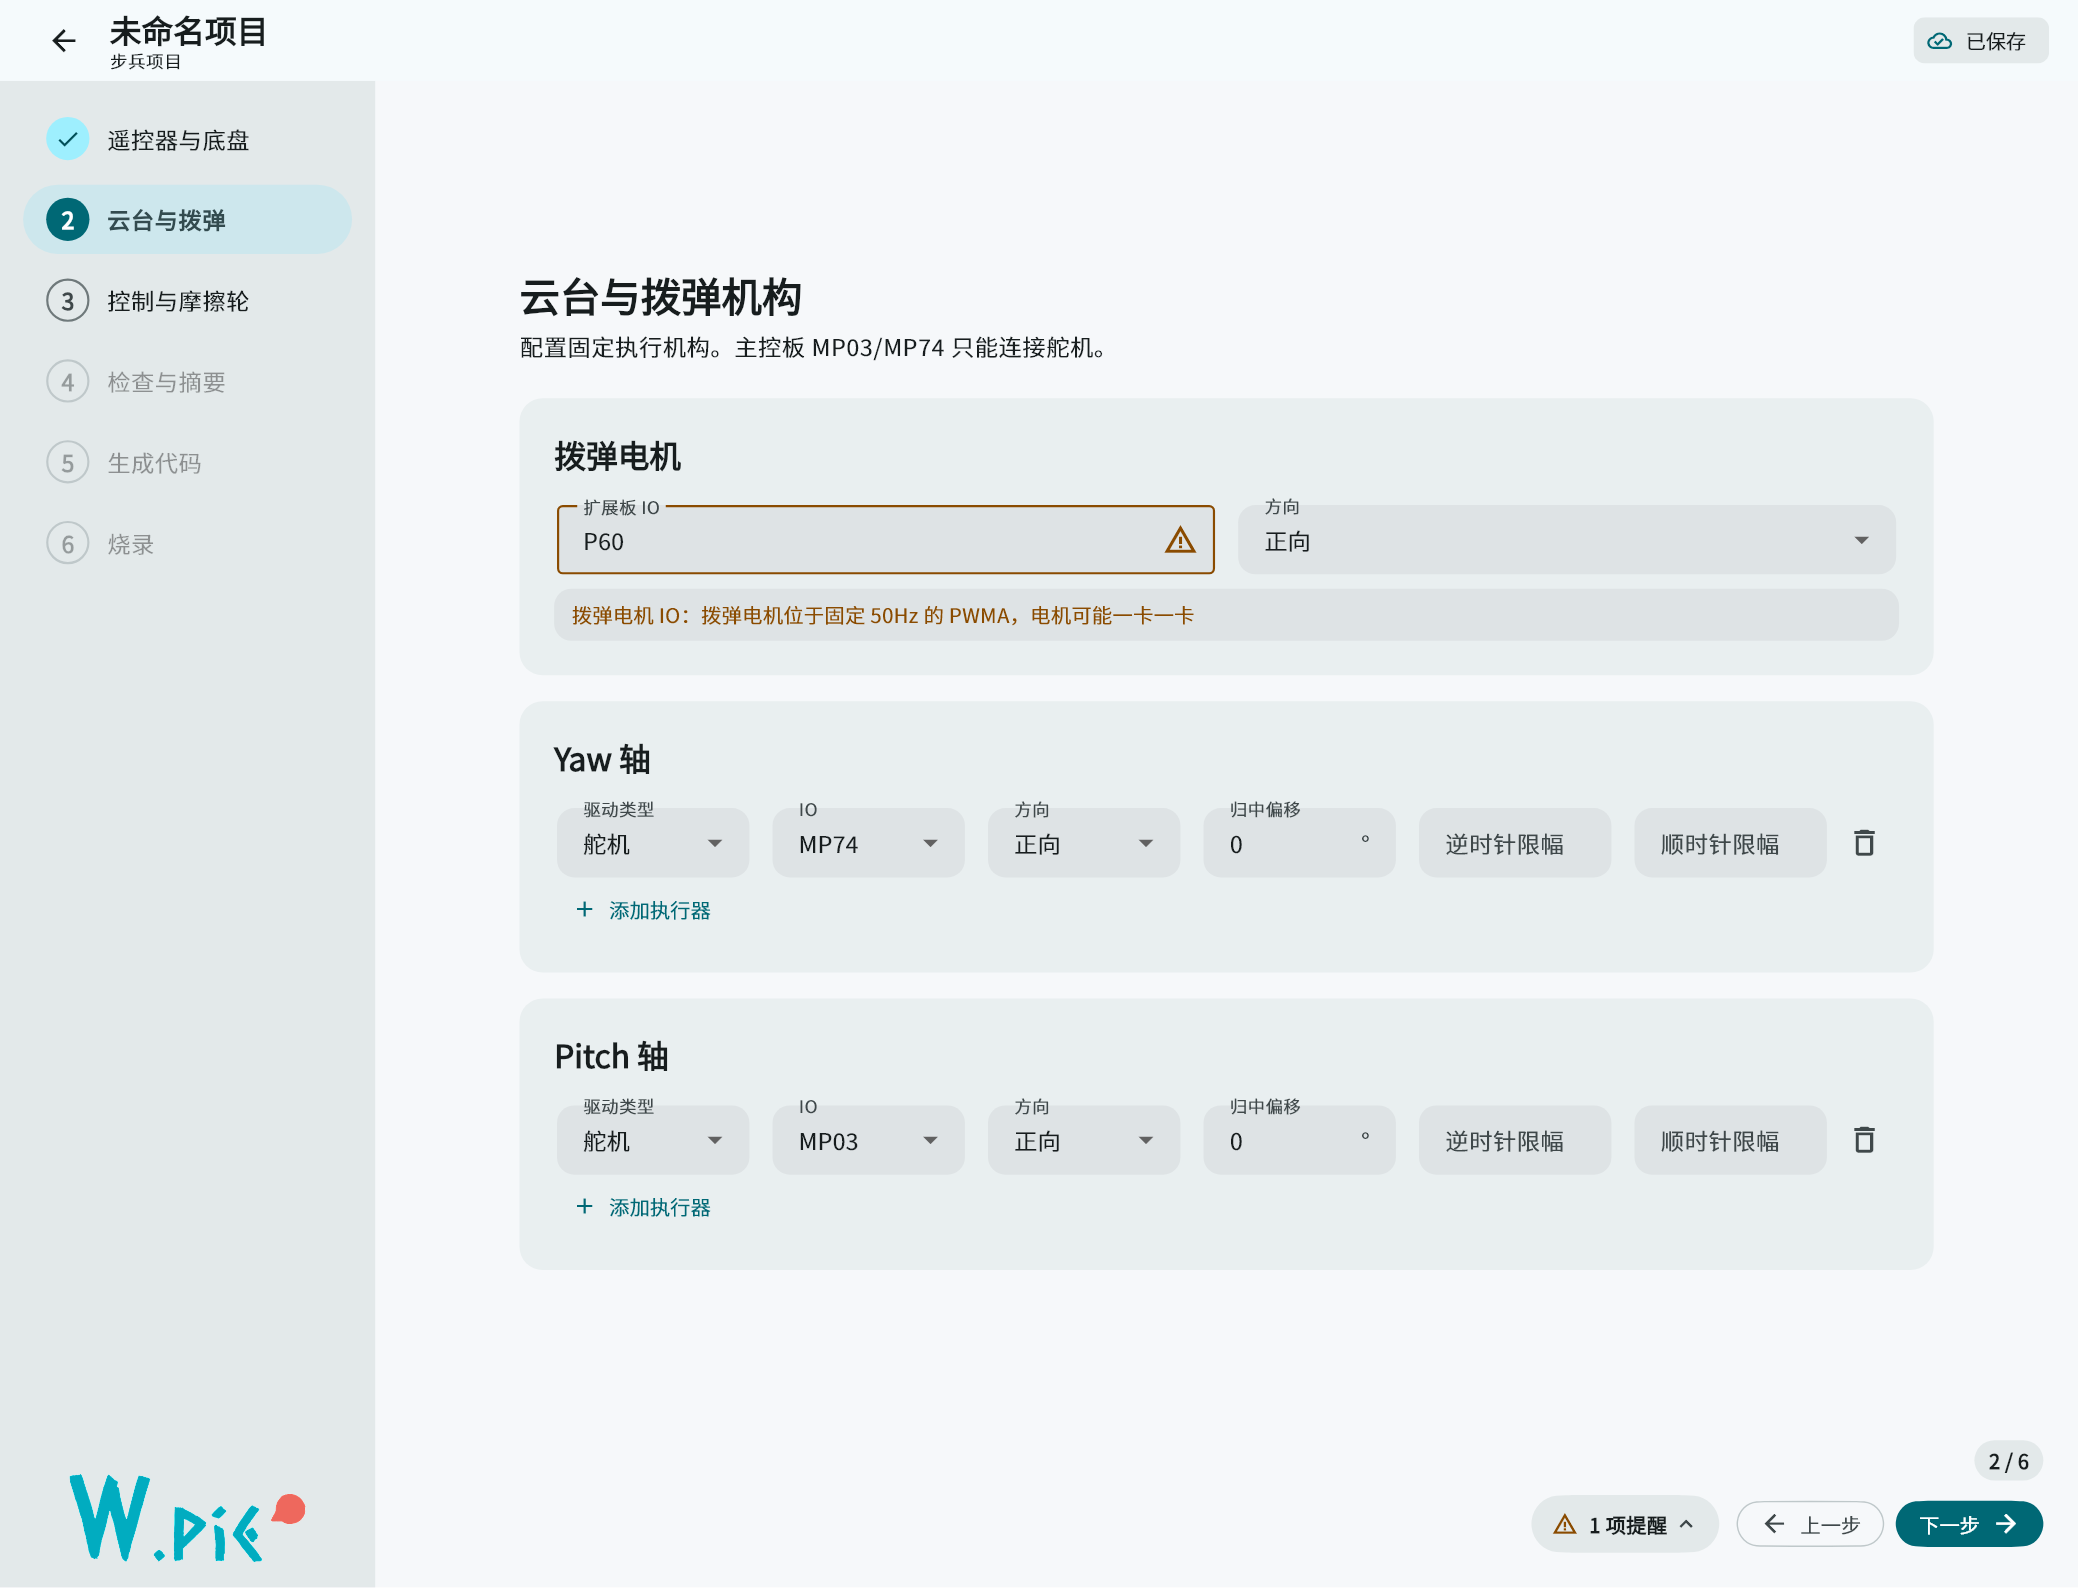
\includegraphics[width=0.98\linewidth]{image/ch04/4-1-mechanism.png}
  \caption{“云台与拨弹”页：拨弹电机、Yaw 轴与 Pitch 轴的执行器参数}
  \label{fig:concise-mechanism}
\end{figure}

\subsection{拨弹电机}

拨弹电机负责把弹丸从弹仓送入摩擦轮。填写 IO 与方向，并选择拨弹模式：

\begin{itemize}
  \item \textbf{阻塞开环单发}：每按一次扳机键，拨弹电机转动一个“单发时长”，送出一颗
        弹丸。单发期间底盘与云台暂停响应，因此单发时长不宜过大，250\,ms 是常用的起始值；
  \item \textbf{目视闭环连续拨弹}：按住扳机键持续拨弹，松开即停，由操作手目视控制节奏。
\end{itemize}

“反向拨弹键”用于卡弹时退弹：按住时按相反方向持续转动，松开立即停止。该键可以留空。

拨弹电机所在的引脚组频率较低，页面可能提示“电机可能一卡一卡”。这属于硬件分组决定的
正常提醒，不是配置错误；适当提高拨弹速度或缩短单发时长可以减轻该现象。

\section{控制与摩擦轮}

\subsection{按键分配}

“控制与摩擦轮”页为拨弹与摩擦轮分配按键（图~\ref{fig:concise-controls}）。同一个数字
按键不能分配给两个动作；启用冲刺后 LC 归底盘使用，启用云台归中后 RC 归云台使用；
方向键按用途占用。冲突会在检查页以错误列出，也可点击条目跳回本页修改。

\begin{figure}[htbp]
  \centering
  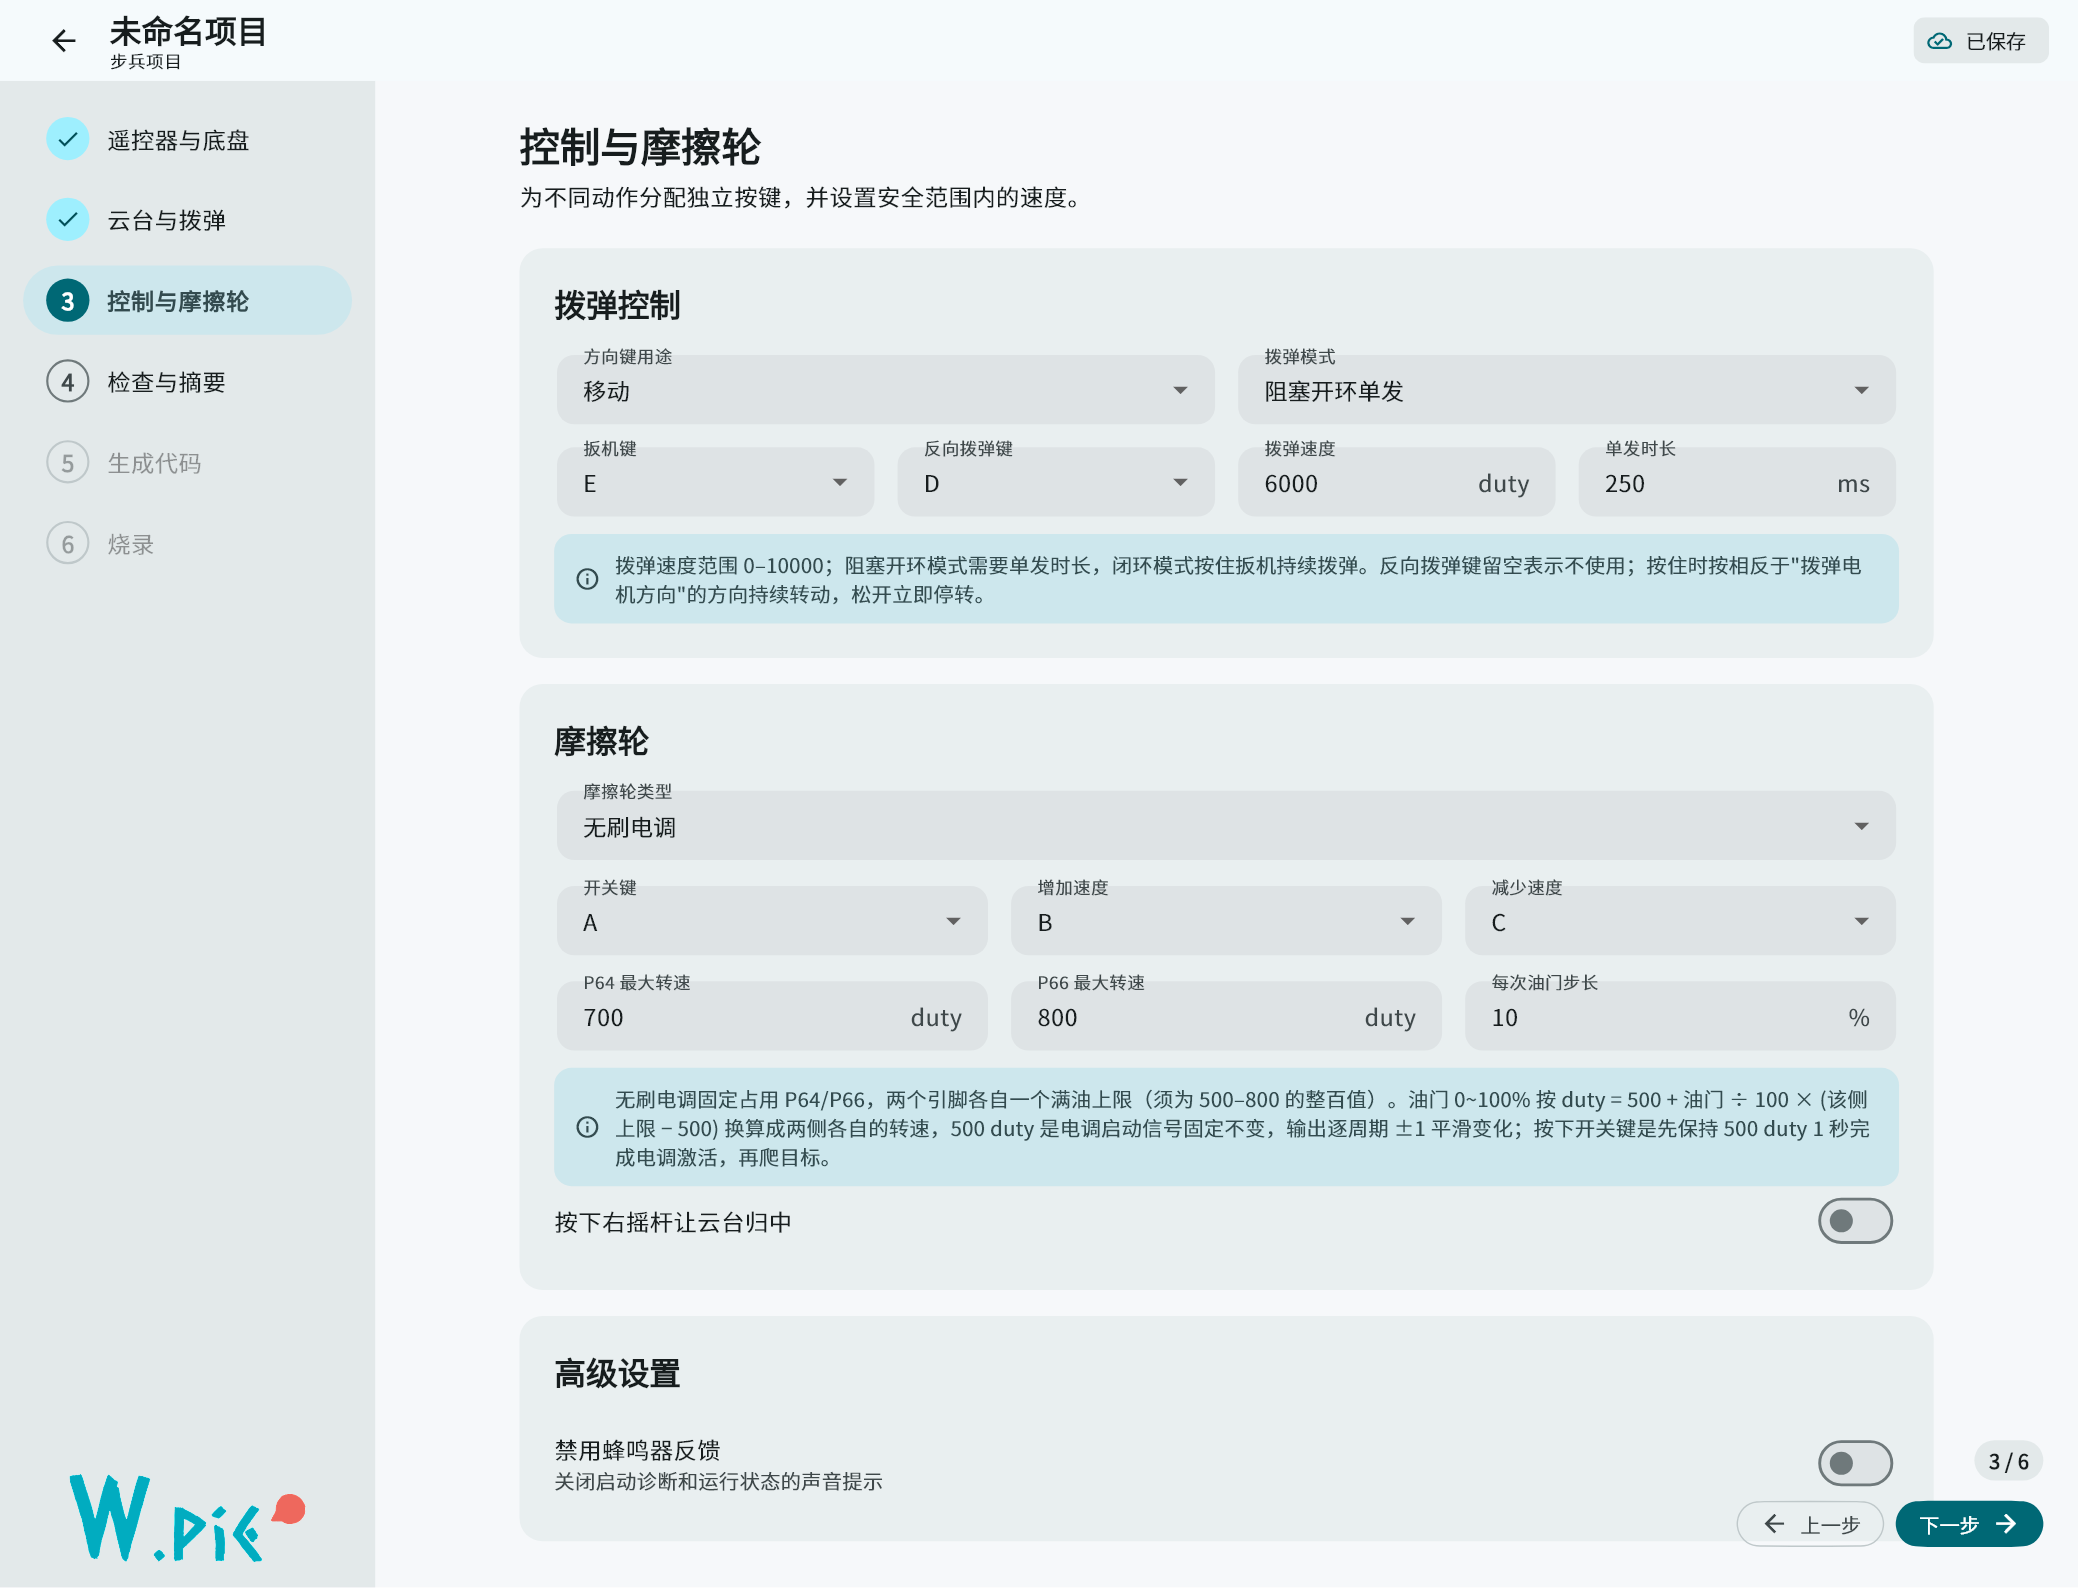
\includegraphics[width=0.98\linewidth]{image/ch04/4-2-controls.png}
  \caption{“控制与摩擦轮”页：拨弹按键与参数、摩擦轮按键与两侧最大转速}
  \label{fig:concise-controls}
\end{figure}

\subsection{摩擦轮}

摩擦轮使用无刷电机与电调，软件把安全规程固化在固件中，界面只暴露油门与最大转速。
摩擦轮类型选择“无刷电调”后固定占用 P64、P66 两个端口；选择“不使用”时释放。

摩擦轮需要三个按键：\textbf{开关键}在停止与当前油门之间切换，\textbf{增加速度键}与
\textbf{减少速度键}按“每次油门步长”调整油门。油门范围为 0--100\%，步长常用 10\%。
两侧分别设置\textbf{最大转速}，取值为 500--800 的整百值，用于补偿两侧机械差异。

摩擦轮的启动与停止由固件按安全流程执行：启动时先以启动转速保持约一秒完成电调激活，
再平滑爬升到目标；停止时沿同一斜坡降回后停止。激活与渐变期间不需要人工干预，也不应在
高速运转时直接切断电源。

两侧最大转速的标定方法：

\begin{enumerate}
  \item 两侧先都填 800，油门步长设为 10\%；
  \item 架空发射机构，人员离开射界，按开关键启动，确认两侧都能平稳起转；
  \item 逐档增加油门，比较两侧声音与弹丸初速；偏慢的一侧适当调高最大转速，或把偏快
        一侧调低；
  \item 确定常用工作点后记录数值，比赛中只调整油门档位，不再修改最大转速。
\end{enumerate}

“高级设置”中的“禁用蜂鸣器反馈”用于关闭上电与状态变化时的提示音，适合安静的调试环境。
该开关不影响摩擦轮的安全流程。

\section{检查、编译与烧录}

三页配置完成后进入“检查与摘要”。除错误外，步兵项目常见的警告包括：冲刺速度低于建议值、
拨弹电机位于低频引脚组、摩擦轮最大转速偏低等。警告不阻止生成，但应逐条确认是否符合
实际方案。

编译与烧录的步骤与第~\ref{ch:concise-debug}~章一致：关闭四个供电开关，主控板断电后
重新连接 USB，检测到设备后点击“编译并烧录”。烧录完成后按附录~\ref{app:concise-check}
的检查单逐项核对，再落地低速试走。

\begin{note}
步兵固件同时驱动底盘、云台、拨弹与摩擦轮。首次上电应架空并清空弹仓；确认底盘方向、
云台行程与摩擦轮启停均正常后，才可安装弹丸并落地运行。
\end{note}
